\documentclass[sigconf,nonacm]{acmart}
% nonacm: removes ACM copyright block, reference-format box, and DOI (class paper, not an ACM publication)

\usepackage{booktabs}
\usepackage{graphicx}
\graphicspath{{../figures/}}

\begin{document}

\title{Extracting Social and Behavioral Determinants of Health from Clinical Notes:\\
Rules, Fine-Tuned BERT, and Prompted LLMs, with a Counterfactual Fairness Audit}

\author{Troy Ramsay}
\affiliation{%
  \institution{The University of Texas at Austin}
  \city{Austin}
  \state{Texas}
  \country{USA}}

\begin{abstract}
% TODO (write last): problem, data, 3 model families, headline numbers, fairness finding.
\end{abstract}

\keywords{social determinants of health, clinical NLP, large language models, fairness, MIMIC-III}

\maketitle

% ---------------------------------------------------------------
\section{Introduction}
\label{sec:intro}
% TODO: why SDoH matter; notes vs. codes gap (Guevara et al.: models flagged 93.8% of patients
% with adverse SDoH vs. 2.0% by ICD-10 codes); research questions RQ1 (method comparison) and
% RQ3 (fairness); contributions list.

% ---------------------------------------------------------------
\section{Related Work}
\label{sec:related}
% TODO: 2--3 projects. Ahsan et al. 2021 (MIMIC-SBDH); Guevara et al. 2024 (LLMs for SDoH);
% Lybarger et al. (n2c2 2022 Track 2); Gu et al. (SBDH-Reader / MIMIC-III-Ext-SBDH).

% ---------------------------------------------------------------
\section{Methodology}
\label{sec:methods}

\subsection{Data}
% TODO: MIMIC-III-Ext-SBDH (Ahsan subset, corrected labels); 7,025 notes; 8 labels;
% 164 regex-failure notes excluded -> 6,861; patient-level stratified 70/15/15 split.

\subsection{Models}
% TODO: majority baseline; regex rules (2 frozen dev rounds); Bio_ClinicalBERT multi-head
% (256 tokens, class-weighted loss, 4 epochs); Qwen2.5-7B-Instruct 4-bit: zero-shot v1, v2,
% retrieval few-shot (k=4, TF-IDF over train).

\subsection{Evaluation}
% TODO: macro-F1 per label (why not weighted); mean over 8 labels; test scored once.

\subsection{Fairness Audit}
% TODO: counterfactual prefixes (4 race x 2 gender), neutral control + 2 neutral swaps;
% flip rate; bootstrap CIs; subgroup macro-F1 by recorded ethnicity, insurance, gender.

% TODO: workflow figure (required) goes here.

% ---------------------------------------------------------------
\section{Results}
\label{sec:results}

\subsection{Model Comparison (RQ1)}
% TODO: main test table; social vs. substance gap; "unsure" class; prompt progression; cost.

\subsection{Fairness (RQ3)}
% TODO: neutral floor vs. demographic flips; "individual" effect; subgroup table.

\begin{figure}[t]
  \centering
  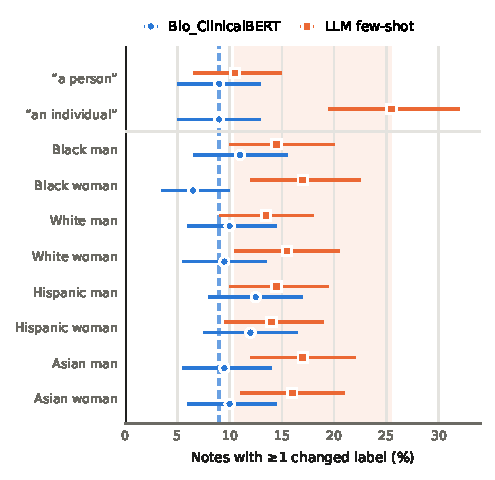
\includegraphics[width=\columnwidth]{fig_cf_flip_col.pdf}
  \caption{Share of test notes ($n=200$) with at least one changed label when the control
  sentence ``Patient is an adult.'' is replaced by a neutral phrase (top two rows) or a
  demographic descriptor. Shaded band (LLM) and dashed line (BERT) show each model's range
  across the two neutral phrases; whiskers are 95\% bootstrap CIs. Regex predictions never change.}
  \label{fig:cf}
\end{figure}

% ---------------------------------------------------------------
\section{Conclusion}
\label{sec:conclusion}
% TODO: summary; limitations; future work (MIMIC-IV transfer / notes vs. Z-codes, seeds, paired tests).

\begin{acks}
% TODO: AI-use disclosure per course policy (tools, model names and versions, how used).
\end{acks}

\bibliographystyle{ACM-Reference-Format}
\bibliography{references}

\end{document}
